% Options for packages loaded elsewhere
\PassOptionsToPackage{unicode}{hyperref}
\PassOptionsToPackage{hyphens}{url}
%
\documentclass[
]{article}
\title{Les prix nobels}
\author{Iris Thorimbert}
\date{07/11/2021}

\usepackage{amsmath,amssymb}
\usepackage{lmodern}
\usepackage{iftex}
\ifPDFTeX
  \usepackage[T1]{fontenc}
  \usepackage[utf8]{inputenc}
  \usepackage{textcomp} % provide euro and other symbols
\else % if luatex or xetex
  \usepackage{unicode-math}
  \defaultfontfeatures{Scale=MatchLowercase}
  \defaultfontfeatures[\rmfamily]{Ligatures=TeX,Scale=1}
\fi
% Use upquote if available, for straight quotes in verbatim environments
\IfFileExists{upquote.sty}{\usepackage{upquote}}{}
\IfFileExists{microtype.sty}{% use microtype if available
  \usepackage[]{microtype}
  \UseMicrotypeSet[protrusion]{basicmath} % disable protrusion for tt fonts
}{}
\makeatletter
\@ifundefined{KOMAClassName}{% if non-KOMA class
  \IfFileExists{parskip.sty}{%
    \usepackage{parskip}
  }{% else
    \setlength{\parindent}{0pt}
    \setlength{\parskip}{6pt plus 2pt minus 1pt}}
}{% if KOMA class
  \KOMAoptions{parskip=half}}
\makeatother
\usepackage{xcolor}
\IfFileExists{xurl.sty}{\usepackage{xurl}}{} % add URL line breaks if available
\IfFileExists{bookmark.sty}{\usepackage{bookmark}}{\usepackage{hyperref}}
\hypersetup{
  pdftitle={Les prix nobels},
  pdfauthor={Iris Thorimbert},
  hidelinks,
  pdfcreator={LaTeX via pandoc}}
\urlstyle{same} % disable monospaced font for URLs
\usepackage[margin=1in]{geometry}
\usepackage{color}
\usepackage{fancyvrb}
\newcommand{\VerbBar}{|}
\newcommand{\VERB}{\Verb[commandchars=\\\{\}]}
\DefineVerbatimEnvironment{Highlighting}{Verbatim}{commandchars=\\\{\}}
% Add ',fontsize=\small' for more characters per line
\usepackage{framed}
\definecolor{shadecolor}{RGB}{248,248,248}
\newenvironment{Shaded}{\begin{snugshade}}{\end{snugshade}}
\newcommand{\AlertTok}[1]{\textcolor[rgb]{0.94,0.16,0.16}{#1}}
\newcommand{\AnnotationTok}[1]{\textcolor[rgb]{0.56,0.35,0.01}{\textbf{\textit{#1}}}}
\newcommand{\AttributeTok}[1]{\textcolor[rgb]{0.77,0.63,0.00}{#1}}
\newcommand{\BaseNTok}[1]{\textcolor[rgb]{0.00,0.00,0.81}{#1}}
\newcommand{\BuiltInTok}[1]{#1}
\newcommand{\CharTok}[1]{\textcolor[rgb]{0.31,0.60,0.02}{#1}}
\newcommand{\CommentTok}[1]{\textcolor[rgb]{0.56,0.35,0.01}{\textit{#1}}}
\newcommand{\CommentVarTok}[1]{\textcolor[rgb]{0.56,0.35,0.01}{\textbf{\textit{#1}}}}
\newcommand{\ConstantTok}[1]{\textcolor[rgb]{0.00,0.00,0.00}{#1}}
\newcommand{\ControlFlowTok}[1]{\textcolor[rgb]{0.13,0.29,0.53}{\textbf{#1}}}
\newcommand{\DataTypeTok}[1]{\textcolor[rgb]{0.13,0.29,0.53}{#1}}
\newcommand{\DecValTok}[1]{\textcolor[rgb]{0.00,0.00,0.81}{#1}}
\newcommand{\DocumentationTok}[1]{\textcolor[rgb]{0.56,0.35,0.01}{\textbf{\textit{#1}}}}
\newcommand{\ErrorTok}[1]{\textcolor[rgb]{0.64,0.00,0.00}{\textbf{#1}}}
\newcommand{\ExtensionTok}[1]{#1}
\newcommand{\FloatTok}[1]{\textcolor[rgb]{0.00,0.00,0.81}{#1}}
\newcommand{\FunctionTok}[1]{\textcolor[rgb]{0.00,0.00,0.00}{#1}}
\newcommand{\ImportTok}[1]{#1}
\newcommand{\InformationTok}[1]{\textcolor[rgb]{0.56,0.35,0.01}{\textbf{\textit{#1}}}}
\newcommand{\KeywordTok}[1]{\textcolor[rgb]{0.13,0.29,0.53}{\textbf{#1}}}
\newcommand{\NormalTok}[1]{#1}
\newcommand{\OperatorTok}[1]{\textcolor[rgb]{0.81,0.36,0.00}{\textbf{#1}}}
\newcommand{\OtherTok}[1]{\textcolor[rgb]{0.56,0.35,0.01}{#1}}
\newcommand{\PreprocessorTok}[1]{\textcolor[rgb]{0.56,0.35,0.01}{\textit{#1}}}
\newcommand{\RegionMarkerTok}[1]{#1}
\newcommand{\SpecialCharTok}[1]{\textcolor[rgb]{0.00,0.00,0.00}{#1}}
\newcommand{\SpecialStringTok}[1]{\textcolor[rgb]{0.31,0.60,0.02}{#1}}
\newcommand{\StringTok}[1]{\textcolor[rgb]{0.31,0.60,0.02}{#1}}
\newcommand{\VariableTok}[1]{\textcolor[rgb]{0.00,0.00,0.00}{#1}}
\newcommand{\VerbatimStringTok}[1]{\textcolor[rgb]{0.31,0.60,0.02}{#1}}
\newcommand{\WarningTok}[1]{\textcolor[rgb]{0.56,0.35,0.01}{\textbf{\textit{#1}}}}
\usepackage{graphicx}
\makeatletter
\def\maxwidth{\ifdim\Gin@nat@width>\linewidth\linewidth\else\Gin@nat@width\fi}
\def\maxheight{\ifdim\Gin@nat@height>\textheight\textheight\else\Gin@nat@height\fi}
\makeatother
% Scale images if necessary, so that they will not overflow the page
% margins by default, and it is still possible to overwrite the defaults
% using explicit options in \includegraphics[width, height, ...]{}
\setkeys{Gin}{width=\maxwidth,height=\maxheight,keepaspectratio}
% Set default figure placement to htbp
\makeatletter
\def\fps@figure{htbp}
\makeatother
\setlength{\emergencystretch}{3em} % prevent overfull lines
\providecommand{\tightlist}{%
  \setlength{\itemsep}{0pt}\setlength{\parskip}{0pt}}
\setcounter{secnumdepth}{-\maxdimen} % remove section numbering
\ifLuaTeX
  \usepackage{selnolig}  % disable illegal ligatures
\fi

\begin{document}
\maketitle

M1 MIASHS, semestre 6\\
Cours de M. CROSETTO, Logiciel spécialisé R

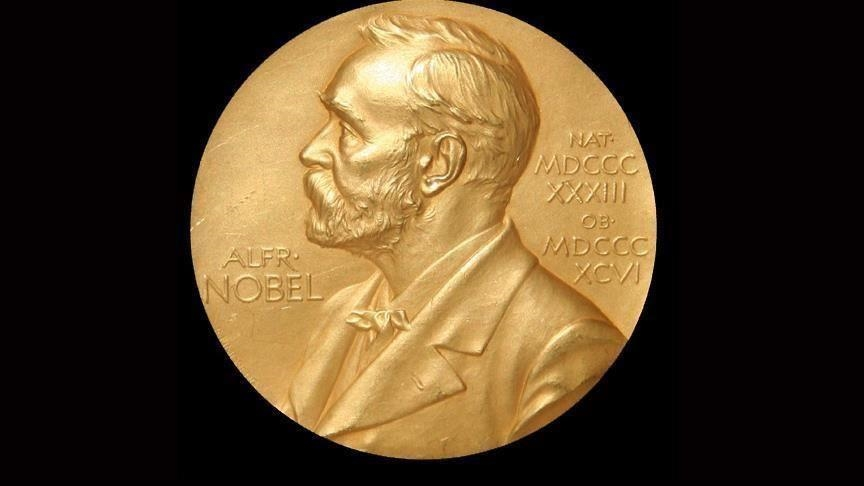
\includegraphics{nobel noir.jpg}

\hypertarget{base-de-donnuxe9es}{%
\subsection{\texorpdfstring{\textbf{Base de
données}}{Base de données}}\label{base-de-donnuxe9es}}

La base de données `Nobel Laureate Publications' est extraite du projet
\emph{TidyTuesday} disponible sur le site \emph{GitHub}. Les données ont
été recueillies par Georgios Karamanis qui s'est appuyé sur différents
sites internets tels que la page officiel du prix nobel, celui des
universités pour récolter et assembler toutes les informations.

Les prix sont décernés chaque année depuis 1901 à des personnes « ayant
apporté le plus grand bénéfice à l'humanité », par leurs inventions,
découvertes et améliorations dans différents domaines.

Le premier tableau, \emph{nobel\_winners}, contient donc, comme son nom
l'indique, le nom des gagnants. Celui-ci est composé de 969 observations
et 18 variables telles que l'année du prix (de 1901 à 2016), la
catégorie (chimie, physique, littérature, médecine, économie et paix),
nom du lauréat, son pays d'origine\ldots{} Dans le second tableau, nommé
\emph{nobel\_winner\_all\_pubs}, nous ai fourni des informations sur les
publications écrites par les gagnants. Nous avons un tableau de 93 394
observations et 11 variables. Ainsi nous pouvons y lire, pour chaque
vainqueurs, le titre et l'année de chacune de ses publications, la revue
dans laquelle elle a été publié, mais également si c'est à partir de ce
papier que l'individu à reçu son prix.

A partir de ces informations, nous pouvons à présent commencer notre
analyse.

Dans un soucis de simplification de la base de données et de son
analyse, j'ai fait le choix de supprimer des données. Tout d'abord j'ai
enlevé toutes les lignes rattachées au prix nobel de la paix. En effet,
j'obtiens de nombreuses valeurs manquantes et de plus, le fait que des
organisations ont parfois été récompensées, cela rend notre analyse plus
complexe. Ensuite, dans un second temps, j'ai supprimé les colonnes
numéro 13, 14 et 15 correspondant respectivement à
\emph{organization\_name}, \emph{organization\_city} et
\emph{organization\_country} car celles-ci entraînentt un doublon de
certain lauréat. C'est donc pour supprimer ces doublons que j'execute la
commande \emph{unique}.

\begin{Shaded}
\begin{Highlighting}[]
\CommentTok{\# nettoyage de la base de données}

\NormalTok{nobel }\OtherTok{\textless{}{-}}\NormalTok{ nobel\_winners }\SpecialCharTok{\%\textgreater{}\%} 
\NormalTok{  .[}\SpecialCharTok{!}\NormalTok{nobel\_winners}\SpecialCharTok{$}\NormalTok{category}\SpecialCharTok{==}\StringTok{"Peace"}\NormalTok{,] }\SpecialCharTok{\%\textgreater{}\%}    \CommentTok{\# suppression de tous les prix associés à Peace}
\NormalTok{  .[}\SpecialCharTok{{-}}\FunctionTok{c}\NormalTok{(}\DecValTok{13}\NormalTok{,}\DecValTok{14}\NormalTok{,}\DecValTok{15}\NormalTok{)]                             }\CommentTok{\# suppression de ces colonnes }

\NormalTok{nobel\_no\_doublon }\OtherTok{\textless{}{-}} \FunctionTok{unique}\NormalTok{(nobel[ }\DecValTok{1}\SpecialCharTok{:}\DecValTok{839}\NormalTok{,])    }\CommentTok{\# suppression des doublons}
\end{Highlighting}
\end{Shaded}

A partir de maintenant nous avons donc 781 observation et 15 variables.

Idée de question

\begin{enumerate}
\def\labelenumi{\arabic{enumi}.}
\tightlist
\item
  combien de pays on gagné le prix nobel quels sont les pays qui ne sont
  plus les memes
\item
  quels sont les 10 pays qui ont recus le plus de prix
\item
  plusieurs fois eu un prix ? et dans deux domaines différents?
\item
  répartition par continent
\item
  nombre de publication avant d'avoir un prix?
\item
  nb ind seul à obtenir le prix et non un travail de groupe? graphe de 1
  , 2 , 3 , 4 , 5 , et plus est ce que le nombre de publication a un
  impact sur la probabilité d'avoir un prix?
\item
  motivation des individus principales? ou tel ou tel type de motiv
\end{enumerate}

\hypertarget{questions}{%
\subsection{\texorpdfstring{\textbf{Questions}}{Questions}}\label{questions}}

\hypertarget{combien-de-femmes-ont-gagnuxe9-un-prix-nobel}{%
\paragraph{\texorpdfstring{\textbf{Combien de femmes ont gagné un prix
nobel?}}{Combien de femmes ont gagné un prix nobel?}}\label{combien-de-femmes-ont-gagnuxe9-un-prix-nobel}}

\begin{Shaded}
\begin{Highlighting}[]
\NormalTok{a }\OtherTok{\textless{}{-}} \FunctionTok{str\_count}\NormalTok{(nobel\_no\_doublon}\SpecialCharTok{$}\NormalTok{gender, }\StringTok{\textquotesingle{}Female\textquotesingle{}}\NormalTok{) }\CommentTok{\#créer une matrice 1 et 0 }
\FunctionTok{sum}\NormalTok{(a,}\AttributeTok{na.rm =}\NormalTok{ T) }\CommentTok{\#compte le nombre de 1}
\end{Highlighting}
\end{Shaded}

\begin{verbatim}
## [1] 33
\end{verbatim}

\hypertarget{quest-ce-que-cela-repruxe9sente-par-rapport-aux-hommes}{%
\paragraph{\texorpdfstring{\textbf{Qu'est-ce que cela représente par
rapport aux
hommes?}}{Qu'est-ce que cela représente par rapport aux hommes?}}\label{quest-ce-que-cela-repruxe9sente-par-rapport-aux-hommes}}

\begin{Shaded}
\begin{Highlighting}[]
\NormalTok{nobel\_no\_doublon }\SpecialCharTok{\%\textgreater{}\%} 
  \FunctionTok{select}\NormalTok{(gender) }\SpecialCharTok{\%\textgreater{}\%} 
  \FunctionTok{ggplot}\NormalTok{()}\SpecialCharTok{+}
  \FunctionTok{aes}\NormalTok{(}\AttributeTok{x =}\NormalTok{ gender, }\AttributeTok{fill =}\NormalTok{ gender)}\SpecialCharTok{+}
  \FunctionTok{geom\_bar}\NormalTok{()}\SpecialCharTok{+}
  \FunctionTok{theme\_classic}\NormalTok{()}\SpecialCharTok{+}
  \FunctionTok{labs}\NormalTok{(}\AttributeTok{title =} \StringTok{"Nombre de prix obtenus en fonction du genre"}\NormalTok{, }\AttributeTok{y =} \StringTok{"Nombre"}\NormalTok{)}\SpecialCharTok{+}
  \FunctionTok{theme}\NormalTok{(}\AttributeTok{plot.title =} \FunctionTok{element\_text}\NormalTok{(}\AttributeTok{hjust =} \FloatTok{0.5}\NormalTok{))}\SpecialCharTok{+}
  \FunctionTok{annotate}\NormalTok{(}\StringTok{"text"}\NormalTok{, }\AttributeTok{x =} \DecValTok{1}\NormalTok{, }\AttributeTok{y =} \DecValTok{65}\NormalTok{, }\AttributeTok{label =} \DecValTok{33}\NormalTok{, }\AttributeTok{color =} \StringTok{\textquotesingle{}\#999999\textquotesingle{}}\NormalTok{)}\SpecialCharTok{+}
  \FunctionTok{annotate}\NormalTok{(}\StringTok{"text"}\NormalTok{, }\AttributeTok{x =} \DecValTok{2}\NormalTok{, }\AttributeTok{y =} \DecValTok{780}\NormalTok{, }\AttributeTok{label =} \DecValTok{748}\NormalTok{, }\AttributeTok{color =} \StringTok{\textquotesingle{}\#999999\textquotesingle{}}\NormalTok{)}
\end{Highlighting}
\end{Shaded}

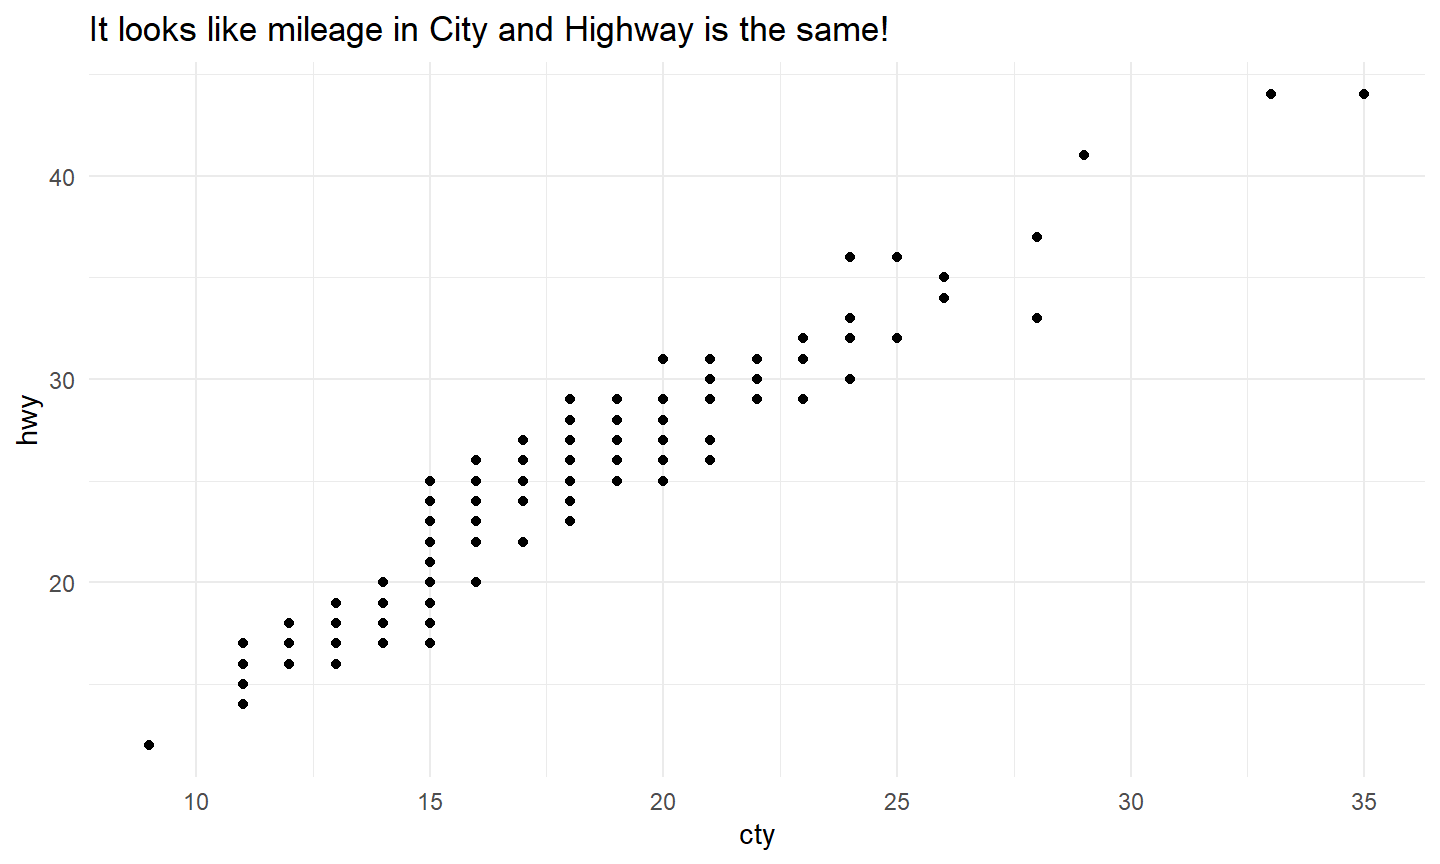
\includegraphics{Thorimbert_Iris_files/figure-latex/unnamed-chunk-4-1.pdf}
\#\#\# \textbf{Qu'est-ce que cela représente en pourcentage?}

\begin{Shaded}
\begin{Highlighting}[]
\NormalTok{pourcentage\_f }\OtherTok{=} \DecValTok{33}\SpecialCharTok{/}\DecValTok{781}\SpecialCharTok{*}\DecValTok{100}
\NormalTok{pourcentage\_h }\OtherTok{=} \DecValTok{748}\SpecialCharTok{/}\DecValTok{781}\SpecialCharTok{*}\DecValTok{100}
\NormalTok{pourcentage\_f }\OtherTok{\textless{}{-}} \FunctionTok{round}\NormalTok{(pourcentage\_f, }\AttributeTok{digits =} \DecValTok{2}\NormalTok{) }\CommentTok{\#2 chiffres après la virgule}
\NormalTok{pourcentage\_h }\OtherTok{\textless{}{-}} \FunctionTok{round}\NormalTok{(pourcentage\_h, }\AttributeTok{digits =} \DecValTok{2}\NormalTok{)}

\CommentTok{\# Création d\textquotesingle{}une table comprennant les pourcentages trouvés au{-}dessus : }
\NormalTok{table }\OtherTok{\textless{}{-}} \FunctionTok{data.frame}\NormalTok{( }\AttributeTok{Sexe =} \FunctionTok{c}\NormalTok{(}\StringTok{"Male"}\NormalTok{, }\StringTok{"Female"}\NormalTok{),}
                     \AttributeTok{Pourcentage =} \FunctionTok{c}\NormalTok{(pourcentage\_h, pourcentage\_f))}

\CommentTok{\#graphique en colonne}
\NormalTok{barre }\OtherTok{\textless{}{-}}\NormalTok{ table }\SpecialCharTok{\%\textgreater{}\%} 
  \FunctionTok{ggplot}\NormalTok{()}\SpecialCharTok{+}
  \FunctionTok{aes}\NormalTok{(}\AttributeTok{x =} \StringTok{""}\NormalTok{,}\AttributeTok{y =}\NormalTok{ Pourcentage, }\AttributeTok{fill =}\NormalTok{ Sexe)}\SpecialCharTok{+}
  \FunctionTok{geom\_col}\NormalTok{()}

\CommentTok{\#transformer en camembert}
\NormalTok{pie }\OtherTok{\textless{}{-}}\NormalTok{ barre }\SpecialCharTok{+}
        \FunctionTok{coord\_polar}\NormalTok{(}\AttributeTok{theta =} \StringTok{"y"}\NormalTok{)}

\CommentTok{\#Mise en page du camembert}
\NormalTok{blank\_theme }\OtherTok{\textless{}{-}} \FunctionTok{theme\_minimal}\NormalTok{() }\SpecialCharTok{+} 
  \FunctionTok{theme}\NormalTok{(}
    \AttributeTok{axis.title.x =} \FunctionTok{element\_blank}\NormalTok{(),}
    \AttributeTok{axis.title.y =} \FunctionTok{element\_blank}\NormalTok{(),}\CommentTok{\#on enleve les nom des axes x et y}
    \AttributeTok{panel.border =} \FunctionTok{element\_blank}\NormalTok{(),}
    \AttributeTok{panel.grid=}\FunctionTok{element\_blank}\NormalTok{(),}
    \AttributeTok{axis.ticks =} \FunctionTok{element\_blank}\NormalTok{())}\SpecialCharTok{+} 
    \FunctionTok{theme}\NormalTok{(}\AttributeTok{axis.text.x =} \FunctionTok{element\_blank}\NormalTok{()) }\CommentTok{\#on enleve les valeurs des axes}

\NormalTok{pie }\SpecialCharTok{+}
\NormalTok{  blank\_theme }\SpecialCharTok{+} \FunctionTok{labs}\NormalTok{(}\AttributeTok{title =} \StringTok{"Nombre de prix obtenus en fonction du genre"}\NormalTok{)}\SpecialCharTok{+}
  \FunctionTok{theme}\NormalTok{(}\AttributeTok{plot.title =} \FunctionTok{element\_text}\NormalTok{(}\AttributeTok{hjust =} \FloatTok{0.5}\NormalTok{))}\SpecialCharTok{+}
  \FunctionTok{geom\_text}\NormalTok{(}\FunctionTok{aes}\NormalTok{(}\AttributeTok{y =}\NormalTok{ Pourcentage}\SpecialCharTok{/}\DecValTok{2} \SpecialCharTok{+} \FunctionTok{c}\NormalTok{(}\DecValTok{0}\NormalTok{, }\FunctionTok{cumsum}\NormalTok{(Pourcentage)[}\SpecialCharTok{{-}}\FunctionTok{length}\NormalTok{(Pourcentage)]),}
                \AttributeTok{label =} \FunctionTok{percent}\NormalTok{(Pourcentage}\SpecialCharTok{/}\DecValTok{100}\NormalTok{)), }\AttributeTok{size=}\FloatTok{3.3}\NormalTok{, }\AttributeTok{color =} \StringTok{\textquotesingle{}black\textquotesingle{}}\NormalTok{) }\CommentTok{\# ajout des chiffres}
\end{Highlighting}
\end{Shaded}

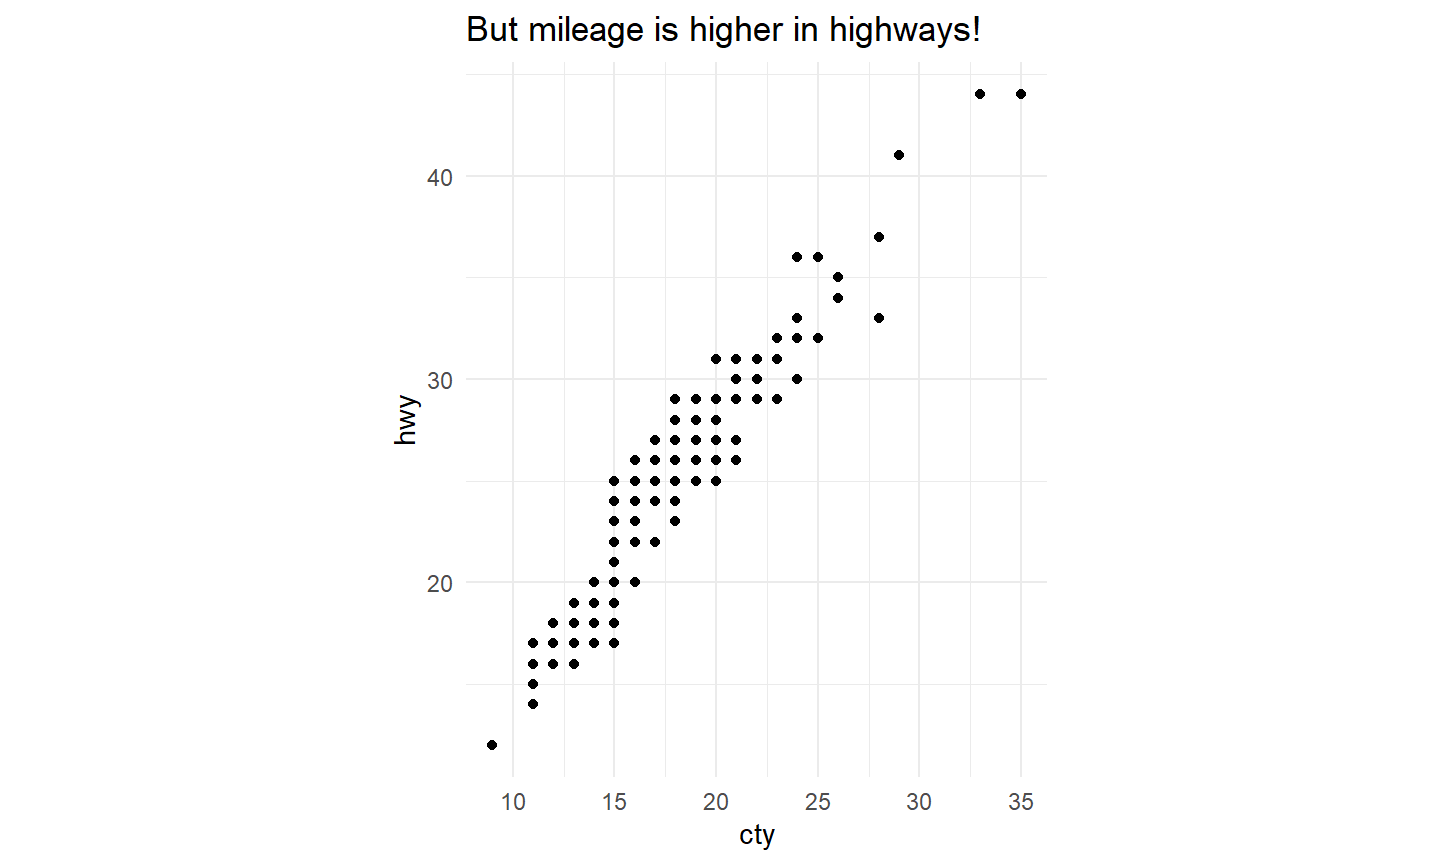
\includegraphics{Thorimbert_Iris_files/figure-latex/unnamed-chunk-5-1.pdf}

\hypertarget{en-quelle-annuxe9e-des-femmes-ont-reuxe7u-un-prix}{%
\subsubsection{\texorpdfstring{\textbf{En quelle année des femmes ont
reçu un
prix}}{En quelle année des femmes ont reçu un prix}}\label{en-quelle-annuxe9e-des-femmes-ont-reuxe7u-un-prix}}

\begin{Shaded}
\begin{Highlighting}[]
\CommentTok{\# création d\textquotesingle{}une base pour faciliter la visualisation }
\NormalTok{femme }\OtherTok{\textless{}{-}}\NormalTok{ nobel\_no\_doublon }\SpecialCharTok{\%\textgreater{}\%} 
  \FunctionTok{filter}\NormalTok{(gender }\SpecialCharTok{==} \StringTok{"Female"}\NormalTok{) }\SpecialCharTok{\%\textgreater{}\%} 
  \FunctionTok{select}\NormalTok{(prize\_year,category, full\_name, prize\_share)}

\NormalTok{nobel\_no\_doublon }\SpecialCharTok{\%\textgreater{}\%} 
  \FunctionTok{filter}\NormalTok{(gender }\SpecialCharTok{==}\StringTok{"Female"}\NormalTok{) }\SpecialCharTok{\%\textgreater{}\%} 
  \FunctionTok{group\_by}\NormalTok{(prize\_year ) }\SpecialCharTok{\%\textgreater{}\%} 
  \FunctionTok{count}\NormalTok{(prize\_year) }\SpecialCharTok{\%\textgreater{}\%}  
  \FunctionTok{ggplot}\NormalTok{(}\FunctionTok{aes}\NormalTok{(}\AttributeTok{x =}\NormalTok{ prize\_year, }\AttributeTok{y=}\NormalTok{n))}\SpecialCharTok{+}
  \FunctionTok{geom\_point}\NormalTok{(}\AttributeTok{color =} \StringTok{"\#FF6666"}\NormalTok{)}\SpecialCharTok{+} 
  \FunctionTok{scale\_x\_continuous}\NormalTok{(}\AttributeTok{breaks =} \FunctionTok{c}\NormalTok{(}\DecValTok{1903}\NormalTok{, }\DecValTok{1911}\NormalTok{, }\DecValTok{1926}\NormalTok{, }\DecValTok{1935}\NormalTok{, }\DecValTok{1945}\NormalTok{, }\DecValTok{1963}\NormalTok{, }\DecValTok{1977}\NormalTok{, }\DecValTok{1986}\NormalTok{, }\DecValTok{1996}\NormalTok{, }\DecValTok{2007}\NormalTok{, }\DecValTok{2014}\NormalTok{),}
                     \AttributeTok{limits =} \FunctionTok{c}\NormalTok{(}\DecValTok{1900}\NormalTok{,}\DecValTok{2016}\NormalTok{))}\SpecialCharTok{+}
  \FunctionTok{scale\_y\_continuous}\NormalTok{(}\AttributeTok{breaks =} \FunctionTok{c}\NormalTok{(}\DecValTok{1}\SpecialCharTok{:}\DecValTok{6}\NormalTok{),}\AttributeTok{limits =} \FunctionTok{c}\NormalTok{(}\DecValTok{0}\NormalTok{,}\DecValTok{6}\NormalTok{))}\SpecialCharTok{+}
  \FunctionTok{theme\_classic}\NormalTok{()}\SpecialCharTok{+}
  \FunctionTok{labs}\NormalTok{(}\AttributeTok{title =} \StringTok{"Nombre de femmes ayant reçu un prix nobel de 1901 à 2016"}\NormalTok{, }\AttributeTok{y =} \StringTok{"nombres"}\NormalTok{)}\SpecialCharTok{+}
  \FunctionTok{theme}\NormalTok{(}\AttributeTok{plot.title =} \FunctionTok{element\_text}\NormalTok{(}\AttributeTok{hjust =} \FloatTok{0.5}\NormalTok{))}\SpecialCharTok{+}
  \FunctionTok{annotate}\NormalTok{(}\StringTok{"text"}\NormalTok{, }\AttributeTok{x =} \DecValTok{2004}\NormalTok{, }\AttributeTok{y =} \FloatTok{2.3}\NormalTok{, }\AttributeTok{label =} \DecValTok{2004}\NormalTok{, }\AttributeTok{color =} \StringTok{\textquotesingle{}\#999999\textquotesingle{}}\NormalTok{, }\AttributeTok{size =} \DecValTok{3}\NormalTok{)}\SpecialCharTok{+}
  \FunctionTok{annotate}\NormalTok{(}\StringTok{"text"}\NormalTok{, }\AttributeTok{x =} \DecValTok{2009}\NormalTok{, }\AttributeTok{y =} \FloatTok{5.3}\NormalTok{, }\AttributeTok{label =} \DecValTok{2009}\NormalTok{, }\AttributeTok{color =} \StringTok{\textquotesingle{}\#999999\textquotesingle{}}\NormalTok{, }\AttributeTok{size =} \DecValTok{3}\NormalTok{)}\SpecialCharTok{+}
  \FunctionTok{annotate}\NormalTok{(}\StringTok{"text"}\NormalTok{, }\AttributeTok{x =} \DecValTok{2015}\NormalTok{, }\AttributeTok{y =} \FloatTok{2.3}\NormalTok{, }\AttributeTok{label =} \DecValTok{2015}\NormalTok{, }\AttributeTok{color =} \StringTok{\textquotesingle{}\#999999\textquotesingle{}}\NormalTok{, }\AttributeTok{size =} \DecValTok{3}\NormalTok{)}
\end{Highlighting}
\end{Shaded}

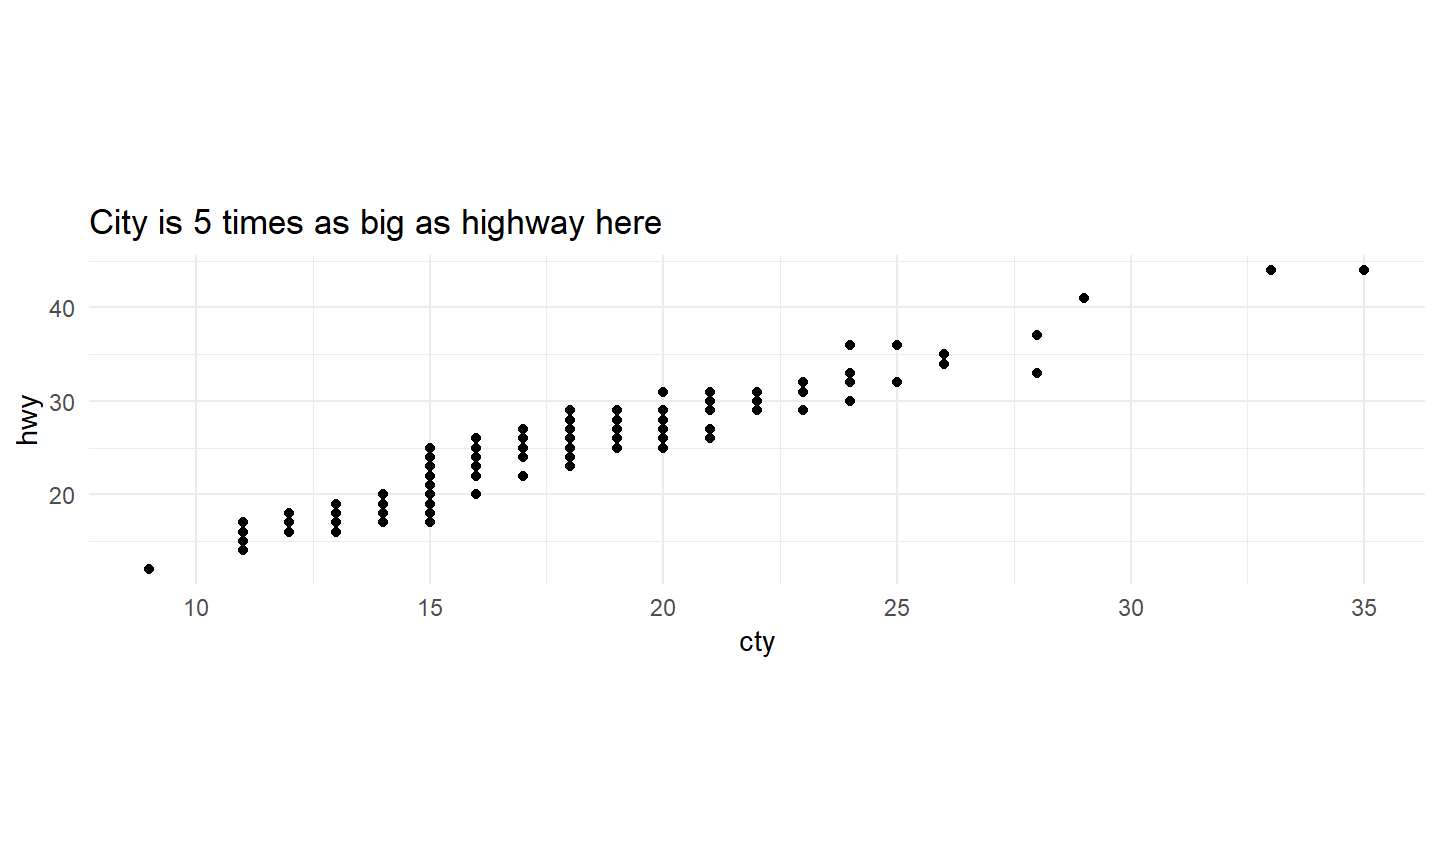
\includegraphics{Thorimbert_Iris_files/figure-latex/unnamed-chunk-6-1.pdf}

\textbf{Remarque :} On peut constater qu'en 2009, 5 femmes ont remporté
un prix. Sachant que nous analysons ici une base pour 5 prix nobels :
chimie, physique, médecine et littérature, économie (puisque nous avons
enlevé le prix nobel de la paix), nous pouvons donc supposer que toutes
les matières ont été gagné par une femme. En revanche, lorsque nous
analysons plus en détail, nous pouvons constater que le prix nobel de
physique a été gagné par un homme. Cela paraît donc étrange et nous fait
interroger sur la véracité de nos résultats. Pourtant la raison est
partfaitement logique : le prix peut être partager par plusieurs
personnes. En effet, nous avons une colonne \emph{prize\_share}, qui
nous permet d'observer avec combien de personne le prix a été partagé.
Ainsi, si l'on revient à l'année 2009, nous sommes en mesure de
constater que le prix nobel de médecine à été partagé entre 3 personnes,
2 femmes et un homme.

\hypertarget{combien-sont-les-individus-qui-partagent-un-prix-uxe0-plusieurs}{%
\paragraph{\texorpdfstring{\textbf{Combien sont les individus qui
partagent un prix à
plusieurs?}}{Combien sont les individus qui partagent un prix à plusieurs?}}\label{combien-sont-les-individus-qui-partagent-un-prix-uxe0-plusieurs}}

\hypertarget{combien-de-nationalituxe9-ont-obtenu-un-prix-nobel}{%
\paragraph{\texorpdfstring{\textbf{Combien de nationalité ont obtenu un
prix
nobel?}}{Combien de nationalité ont obtenu un prix nobel?}}\label{combien-de-nationalituxe9-ont-obtenu-un-prix-nobel}}

\begin{Shaded}
\begin{Highlighting}[]
\NormalTok{nobel\_no\_doublon }\SpecialCharTok{\%\textgreater{}\%} 
  \FunctionTok{select}\NormalTok{(birth\_country) }\SpecialCharTok{\%\textgreater{}\%} 
  \FunctionTok{unique}\NormalTok{() }\SpecialCharTok{\%\textgreater{}\%} 
  \FunctionTok{count}\NormalTok{()}
\end{Highlighting}
\end{Shaded}

\begin{verbatim}
## # A tibble: 1 x 1
##       n
##   <int>
## 1   104
\end{verbatim}

Nous avons donc 104 nationalités différentes qui ont un jour gagné un
prix nobel. Sachant qu'il y a 195 pays dans le monde, environ un pays
sur 2 a un jour été récompensé. Cependant ce résultat est également à
prendre à la légère car nous prenons ici le pays de naissance du
lauréat, or certain individu ont, entre temps, changer de nationnalité.
Nous pouvons par exemple prendre Marie Curie, né en Pologne puis
naturalisée française après son mariage.\\
De plus, comme notre base de donnée commence au début du 20ème siècle,
nous avons des pays qui aujoud'hui n'existe plus et qui entraine une
augmentation du nombre de pays ayant gagné un prix.

\begin{Shaded}
\begin{Highlighting}[]
\NormalTok{nobel\_no\_doublon }\SpecialCharTok{\%\textgreater{}\%} 
  \FunctionTok{select}\NormalTok{(birth\_country) }\SpecialCharTok{\%\textgreater{}\%} 
  \FunctionTok{filter}\NormalTok{(birth\_country }\SpecialCharTok{==} \StringTok{"Prussia (Poland)"}\SpecialCharTok{|}\NormalTok{ birth\_country }\SpecialCharTok{==} \StringTok{"Prussia (Germany)"}\SpecialCharTok{|}\NormalTok{ birth\_country }\SpecialCharTok{==} \StringTok{"Prussia (Russia)"}\NormalTok{) }\SpecialCharTok{\%\textgreater{}\%}  
  \FunctionTok{unique}\NormalTok{()}
\end{Highlighting}
\end{Shaded}

\begin{verbatim}
## # A tibble: 3 x 1
##   birth_country    
##   <chr>            
## 1 Prussia (Poland) 
## 2 Prussia (Germany)
## 3 Prussia (Russia)
\end{verbatim}

\hypertarget{combien-de-personnes-ont-obtenu-plusieurs-prix-nobels}{%
\subsubsection{\texorpdfstring{\textbf{Combien de personnes ont obtenu
plusieurs prix
nobels?}}{Combien de personnes ont obtenu plusieurs prix nobels?}}\label{combien-de-personnes-ont-obtenu-plusieurs-prix-nobels}}

\end{document}
